\section*{Appendix E -- Double Gauss simulations}



Same results but for DG

\subsection{No Delay}

877 retained


\begin{figure}[H]
\centering
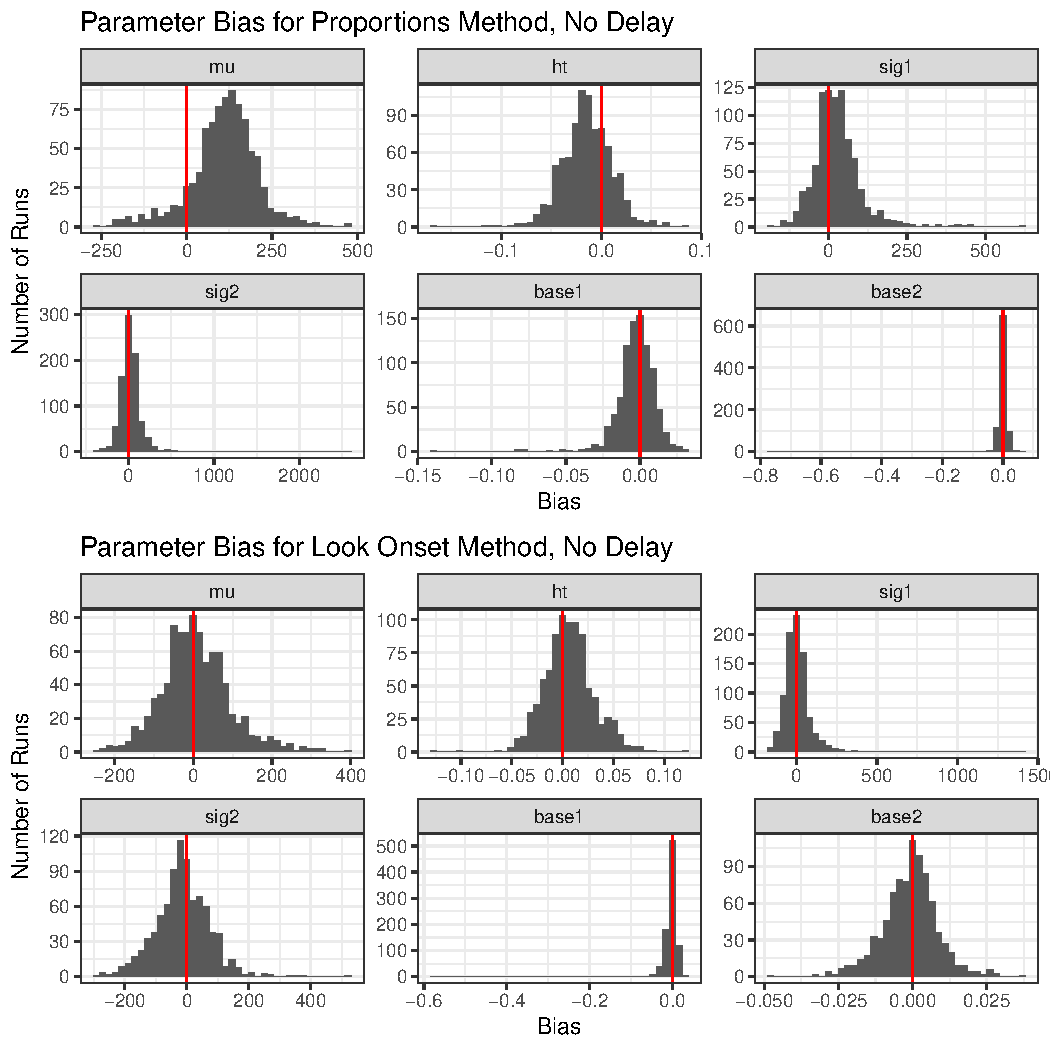
\includegraphics[width=0.9\textwidth]{dg_no_delay_par_bias.pdf}
\caption{Parameter bias for no oculmotor delay}
\label{fig:dg_par_bias_no_delay}
\end{figure}

\begin{figure}[H]
\centering
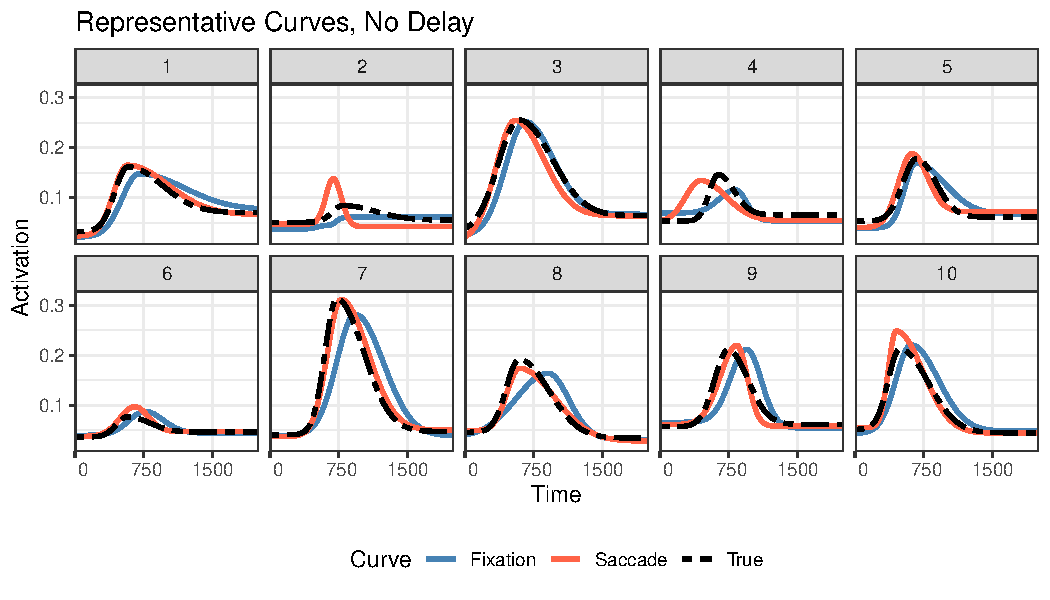
\includegraphics[width=0.9\textwidth]{dg_rep_curves_no_delay.pdf}
\caption{Representative curves for no oculmotor delay}
\label{fig:dg_rep_curves_no_delay}
\end{figure}


\subsection{Uniform Delay}

844 retained


\begin{figure}[H]
\centering
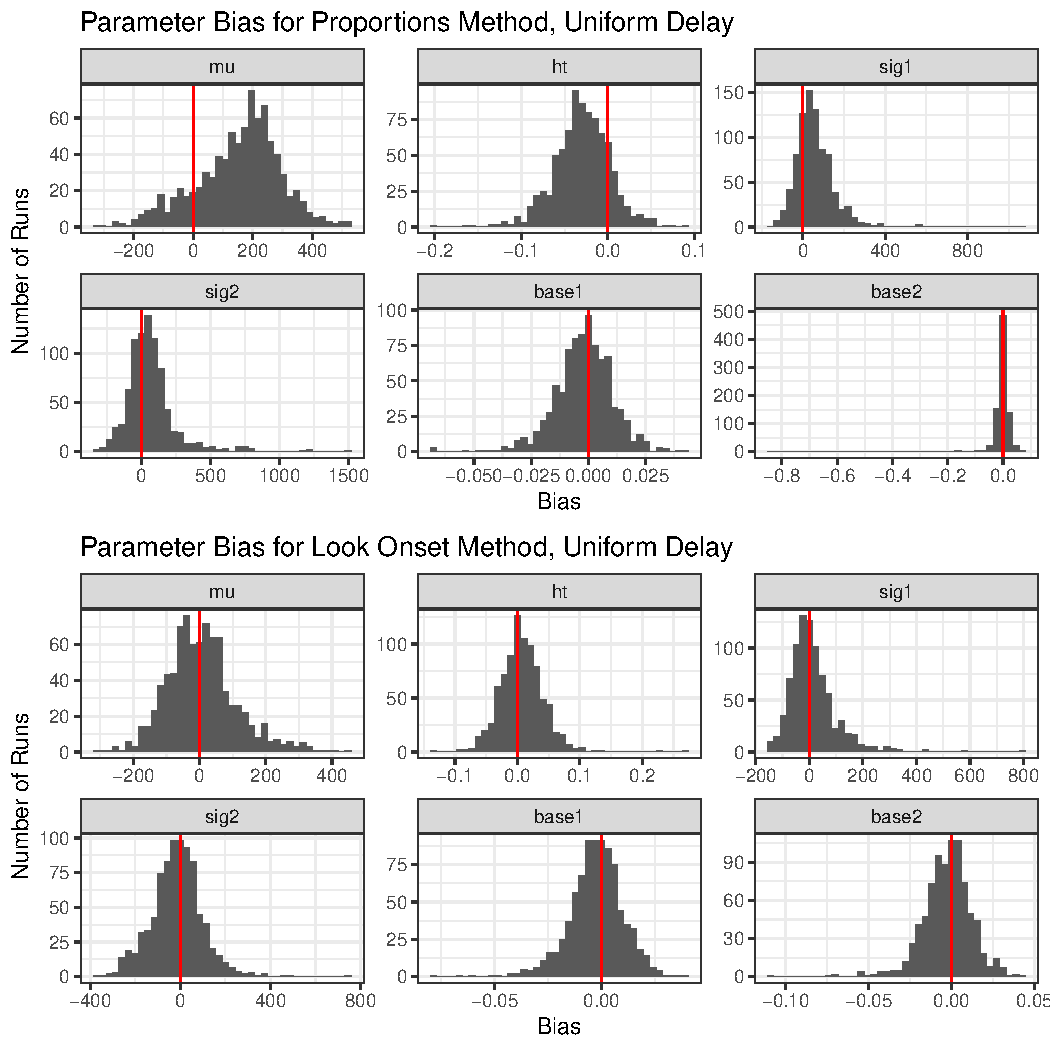
\includegraphics[width=0.9\textwidth]{dg_uniform_delay_par_bias.pdf}
\caption{Parameter bias for uniform OM delay}
\label{fig:dg_par_bias_uniform_delay}
\end{figure}

\begin{figure}[H]
\centering
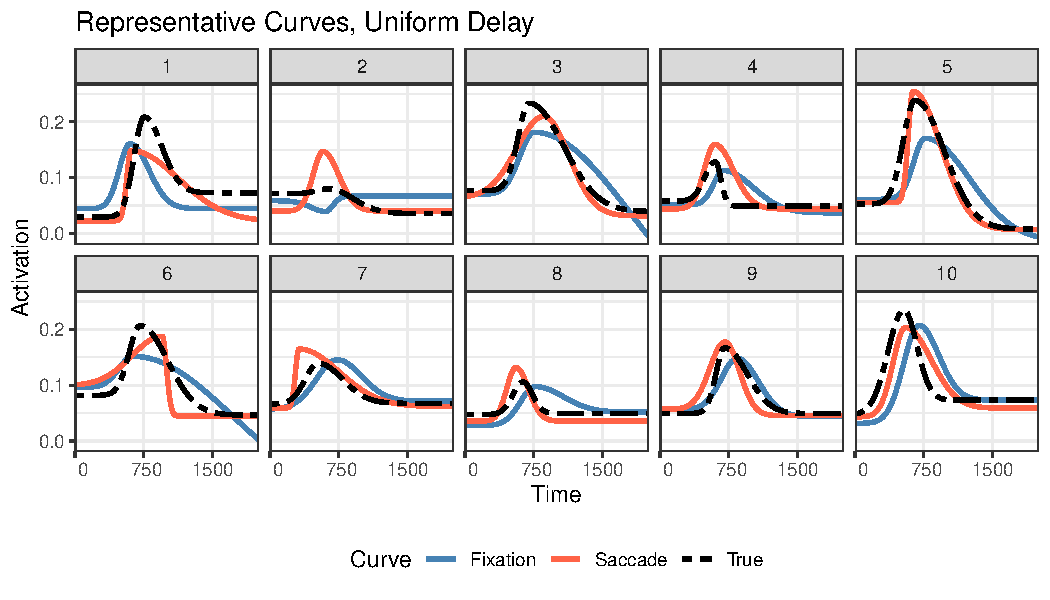
\includegraphics[width=0.9\textwidth]{dg_rep_curves_uniform_delay.pdf}
\caption{Representative curves for uniform oculmotor delay}
\label{fig:dg_rep_curves_uniform_delay}
\end{figure}

\subsection{Weibull Delay}

861 retained

\begin{figure}[H]
\centering
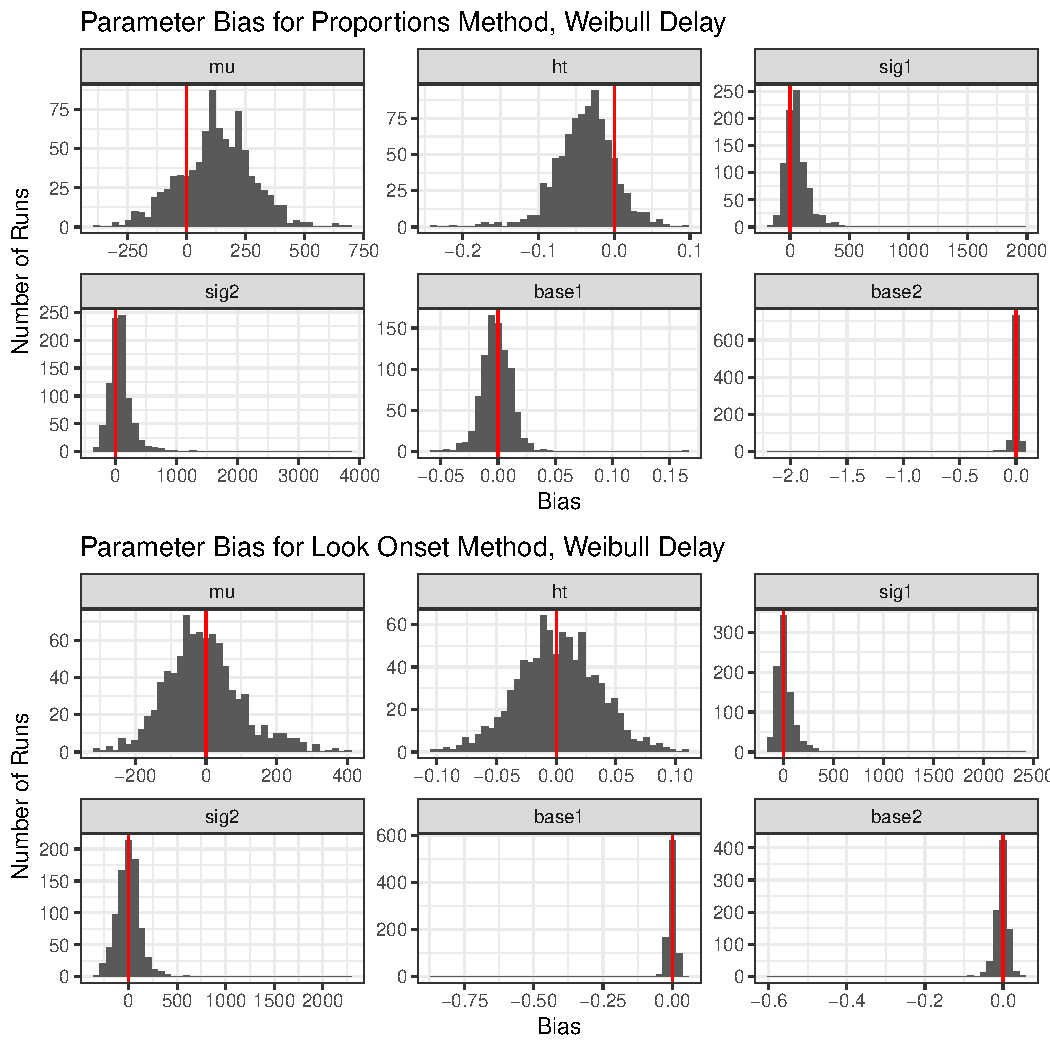
\includegraphics[width=0.9\textwidth]{dg_weibull_delay_par_bias.pdf}
\caption{Parameter bias for weibull OM delay}
\label{fig:dg_par_bias_weibull_delay}
\end{figure}

\begin{figure}[H]
\centering
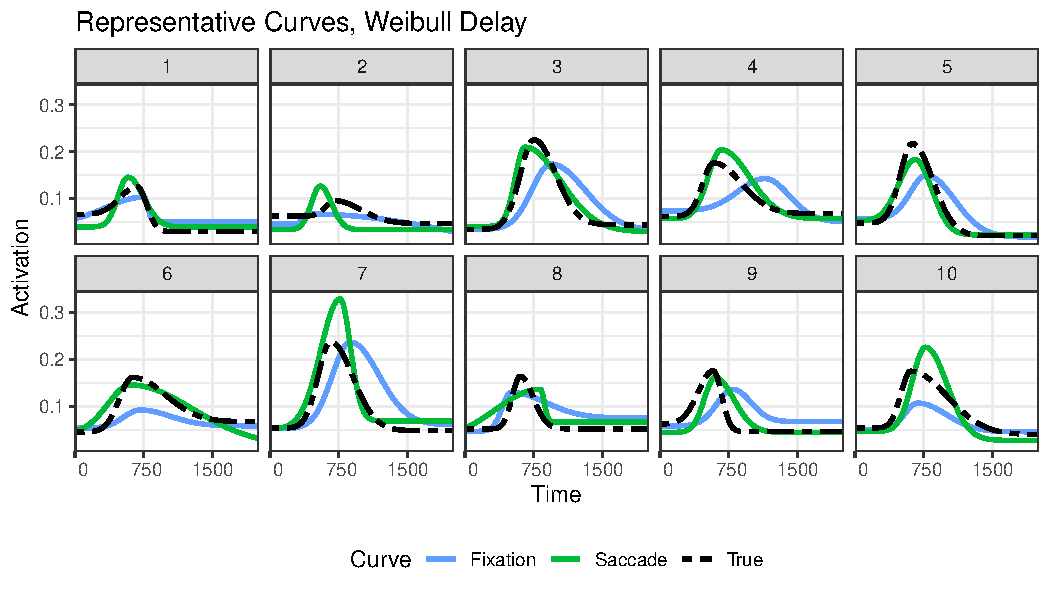
\includegraphics[width=0.9\textwidth]{dg_rep_curves_weibull_delay.pdf}
\caption{Representative curves for weibull oculmotor delay}
\label{fig:dg_rep_curves_weibull_delay}
\end{figure}

\subsection{Results}

\begin{table}[ht]
\centering
\begin{tabular}{llrrrrrr}
  \hline
Curve & Delay & Min. & 1st Qu. & Median & Mean & 3rd Qu. & Max. \\ 
  \hline
Look Onset & No Delay & 0.03 & 0.20 & 0.35 & 0.48 & 0.59 & 5.07 \\ 
  Look Onset & Uniform Delay & 0.03 & 0.43 & 0.73 & 0.91 & 1.18 & 5.71 \\ 
  Look Onset & Weibull Delay & 0.06 & 0.49 & 0.80 & 1.00 & 1.29 & 8.20 \\ 
  Proportion & No Delay & 0.01 & 0.74 & 1.29 & 1.53 & 2.03 & 7.35 \\ 
  Proportion & Uniform Delay & 0.05 & 1.27 & 2.25 & 2.73 & 3.69 & 12.26 \\ 
  Proportion & Weibull Delay & 0.04 & 1.07 & 2.02 & 2.64 & 3.60 & 14.57 \\ 
   \hline
\end{tabular}
\caption{Figures not as striking as logistic, but keep in mind that the scale of this is significantly smaller, peaking at around 0.15 and being close to zero elsewhere. $R^2$ is another metric available that }
\label{tab:dg_mise_sims}
\end{table}

\section*{$R^2$ instead of MISE for logistic/doublegauss}'

The ``minimum" for all of these is like -40 to -100, so mean is also not great for showing.

\subsubsection{for logistic}

\begin{table}[H]
\centering
\begin{tabular}{llrrr}
  \hline
Curve & Delay & 1st Qu. & Median & 3rd Qu. \\ 
  \hline
Look Onset & No Delay & 0.82 & 0.91 & 0.95 \\ 
  Look Onset & Uniform Delay & 0.61 & 0.80 & 0.90 \\ 
  Look Onset & Weibull Delay & 0.58 & 0.79 & 0.89 \\ 
  Proportion & No Delay & 0.52 & 0.66 & 0.75 \\ 
  Proportion & Uniform Delay & 0.11 & 0.40 & 0.58 \\ 
  Proportion & Weibull Delay & 0.16 & 0.42 & 0.63 \\ 
   \hline
\end{tabular}
\caption{$R^2$ for logistic, not as clear a hierarchy}
\label{tab:r2_logistic_sims}
\end{table}

\subsubsection{for doublegauss}

\begin{table}[H]
\centering
\begin{tabular}{llrrr}
  \hline
Curve & Delay & 1st Qu. & Median & 3rd Qu. \\ 
  \hline
Look Onset & No Delay & 0.82 & 0.91 & 0.95 \\ 
  Look Onset & Uniform Delay & 0.61 & 0.80 & 0.90 \\ 
  Look Onset & Weibull Delay & 0.58 & 0.79 & 0.89 \\ 
  Proportion & No Delay & 0.52 & 0.66 & 0.75 \\ 
  Proportion & Uniform Delay & 0.11 & 0.40 & 0.58 \\ 
  Proportion & Weibull Delay & 0.16 & 0.42 & 0.63 \\ 
   \hline
\end{tabular}
\caption{$R^2$ for double gauss}
\label{tab:r2_dg_sims}
\end{table}
